\chapter{PG LDPC (7,3) Implementation using NoC}
\label{chapter7}
This chapter describes the detailed overview of LDPC (7,3) implementation on NoC Mesh 4 $\times$ 4, and comparison of implementation in partitioned and un-partitioned NoC in terms of speed, scalability and overall performance. 
PG-LDPC (7,3) architecture consists of 7 bit-nodes and 7 check-nodes. The block (7,3) indicates
that 7 is the code length and 3 is the number of data bits. 

\section{Implementation Details}

\subsection{Bit-node implementation}
Apart from performing the computation, bit-node has to take care of sending and 
receiving of valid flit from NoC as a processing element.
State diagram and architecture of Bit-node is shown in Figure-\ref{bit_node_fsm}
and Figure-\ref{bit_node_architecture} respectively. 

 Figure \ref{bit_node_architecture} shows the Bit-node architecture. Upon receiving the start signal, bit-node transmits the initial data to check-node via Router. As it receives the data from the check-node, it performs the summation of the incoming signal and then subtracts the corresponding signal. This is equivalent to passing the summation of remaining two data. This value is stored in the register and transmitted as soon as they are calculated. Function of each state is as follow:\\
 \textbf{IDLE}: Power\_on/Reset state. And after complete computation,bit-node enters in this state.\\
 \textbf{SEND\_u0}: As soon as $start/bypass\_LLR= 1$, Bit-node enters into this state and sends $u0$ bits to 3 check-nodes.\\  
 \textbf{DATA\_RCV}: (Data Receive) It waits for $v$ data from check-node and remains in this state until $3$ valid data are received.\\
 \textbf{COMPUTATION}: when all 3 valid flits are received, bit-node performs computation and result is available and stored in u\_register.\\
 \textbf{DATA\_SEND}: After completing the computation, bit-node enters in this state and sends 3 data- flits containing u.\\   
 
\begin{figure} [H]
  \centering
   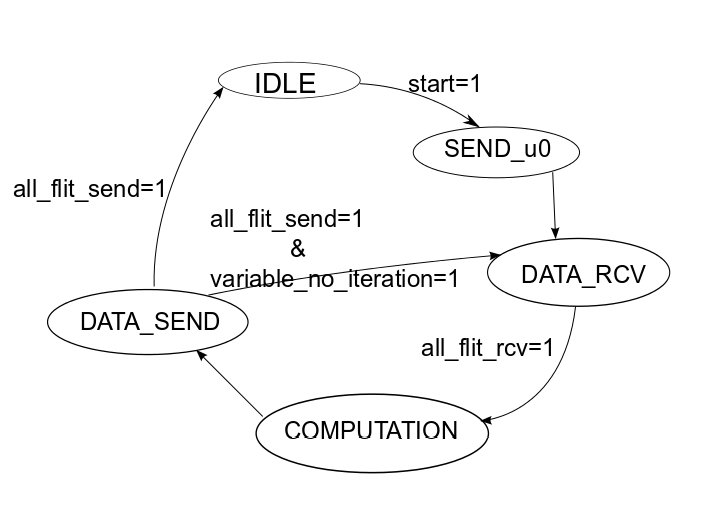
\includegraphics[scale=0.4]{./figs/bit_node_fsm}
  \caption{Bit-node FSM}
  \label{bit_node_fsm}
\end{figure}
  
\begin{figure} [H]
  \centering
   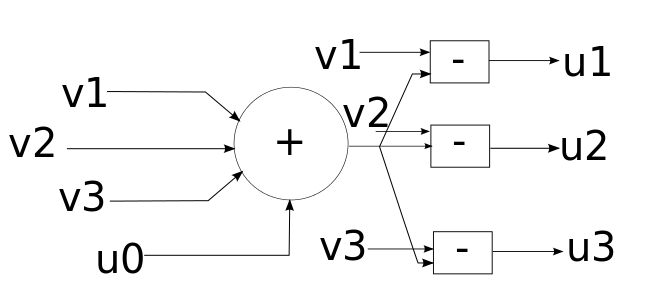
\includegraphics[scale=0.4]{./figs/bit_node}
  \caption{Bit-node Architecture}
  \label{bit_node_architecture}
\end{figure}

 \begin{figure} [H]
  \centering
  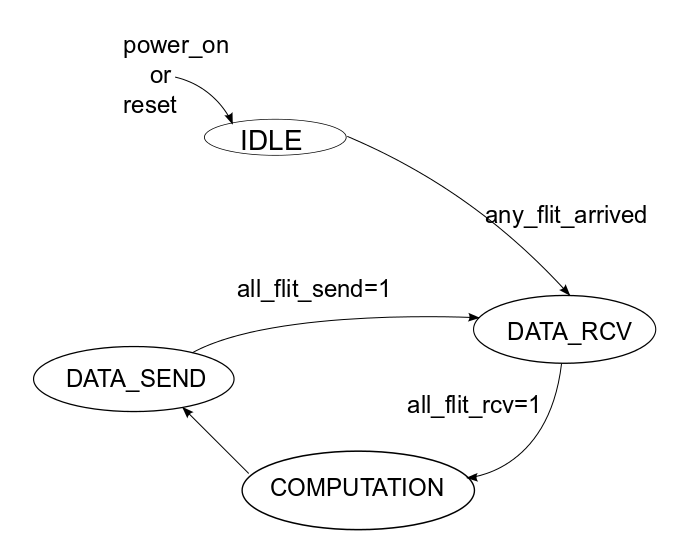
\includegraphics[scale=0.4]{./figs/check_node_fsm}
  \caption{Check-node FSM}
  \label{check_node_fsm}
\end{figure}
 
\begin{figure} [H]
  \centering
  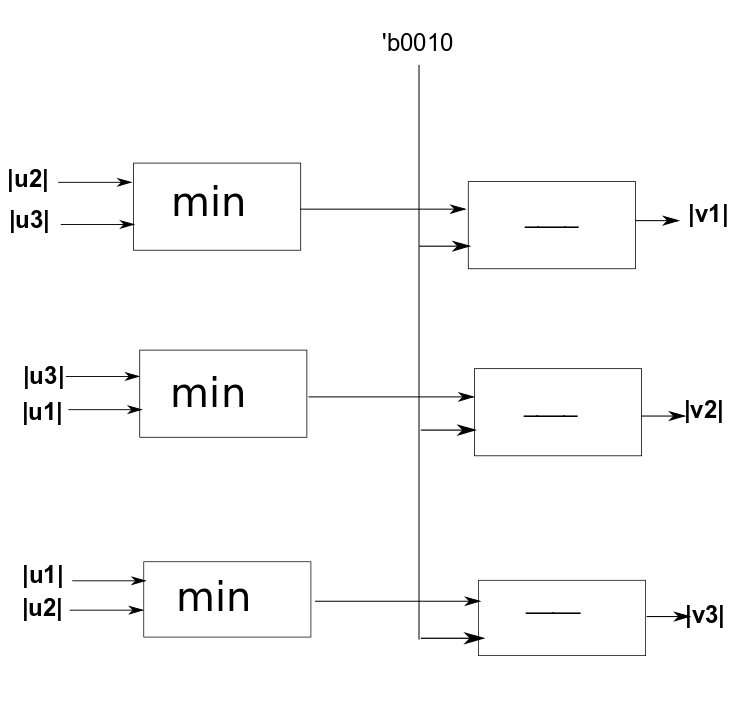
\includegraphics[scale=0.4]{./figs/check_node_mag}
  \caption{Check-node Magnitude Calculation}
  \label{check_node_mag}
\end{figure}

\begin{figure} [H]
  \centering
  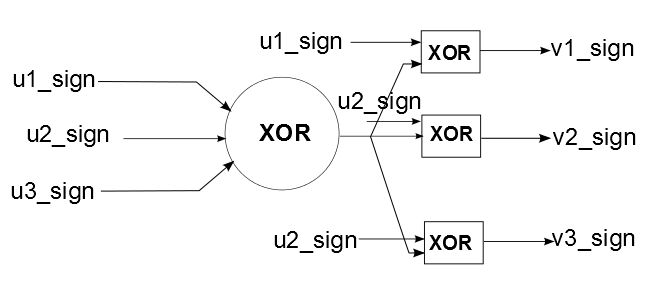
\includegraphics[scale=0.4]{./figs/check_node_sign}
  \caption{Check-node Sign Calculation}
  \label{check_node_sign}
\end{figure}

\begin{figure} [H]
  \centering
   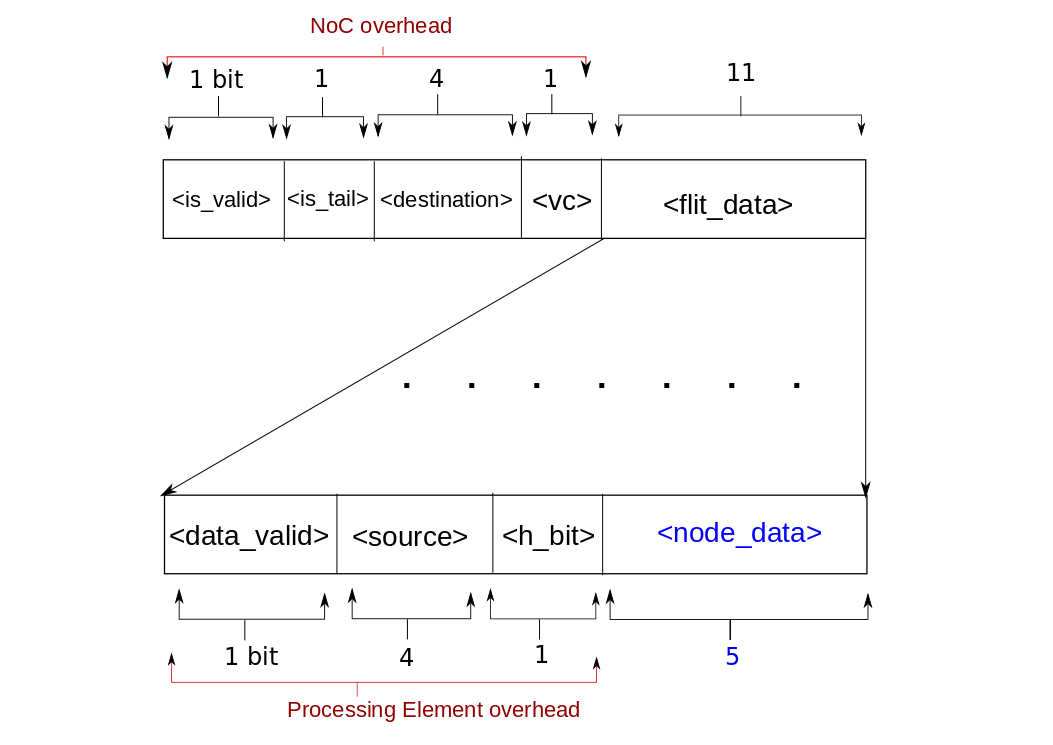
\includegraphics[scale=0.3]{./figs/flit_structure_ldpc_7x7}
  \caption{Data Flit used in PG-LDPC (7,3) on NoC}
  \label{flit_structure_ldpc_7x7}
\end{figure}

 \begin{figure} [H]
  \centering
   \includegraphics[scale=0.3]{./figs/ldpc_7x7_NoC_mesh_4x4}
  \caption{PG-LDPC (7,3) implemented on Mesh 4 $\times$ 4 Un-Partitioned NoC}
  \label{ldpc_7x7_NoC_mesh_4x4}
\end{figure}

 \begin{figure} [H]
  \centering
   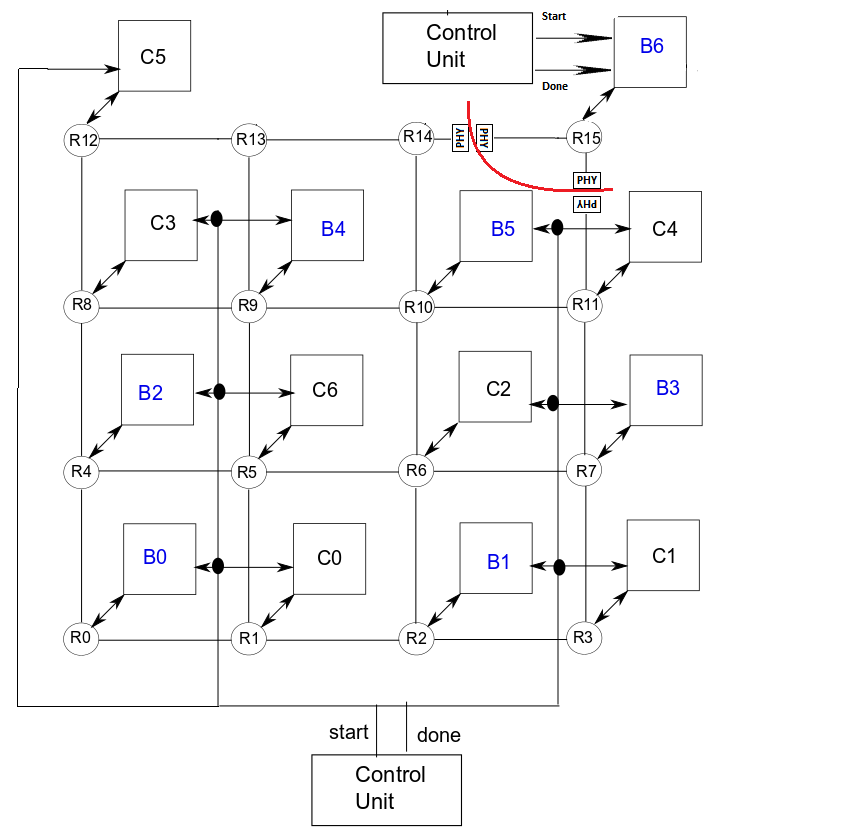
\includegraphics[scale=0.4]{./figs/Partitioned4x4Mesh}
  \caption{PG-LDPC (7,3) implemented on Mesh 4 $\times$ 4 Partitioned NoC}
  \label{Partitioned4x4Mesh}
\end{figure}

 \subsection{System level implementation and comparison of PG-LDPC on an \textit{partitioned} and \textit{un-partitioned} NoC}
 Bit-node and check-node are connected to router one-to-one basis in both partitioned and un-partitioned NoC. 
 Initially the placement is done heuristically. 
 (B-C-B-C) in row and column both sequentially. 
 After careful analysis of worst-case and average communication overhead 
 analysis, the given placement of Bit-node and Check-node is performed. 

 The data sent to NoC must contain additional information called as payload.
 The typical flit structure for this system is shown in the Figure-\ref{flit_structure_ldpc_7x7}.
 The flit contain NoC overhead as well as processing element overhead which is required to arrange 
 the data properly, which are received in random order.
 
Overall system implementation is shown in Figure- \ref{ldpc_7x7_NoC_mesh_4x4} for un-partitioned Mesh NoC and Figure- \ref{Partitioned4x4Mesh} for partitioned Mesh NoC including placement of bit-node and check-node as discussed in \cite{shaishav_mtp}.

 \section{Compilation Results}
 \subsection{Simulation Readings and Comparison}
PG-LDPC (7,3) Decoder is implemented on both a) Mesh 4 $\times$ 4 partitioned NoC and b) Mesh 4 $\times$ 4 un-partitioned NoC. Simulation results are checked and verified for correctness. Both the results are matching with correct one.

\begin{table} [H]
\caption{Results for LDPC 7x7 on partitioned and un-partitioned NoC}
\begin{center}
\begin{tabular}{||c || c| c ||} \hline
	Parameters 			      	& LDPC on 4 $\times$ 4      	& LDPC on 4 $\times$ 4 					\\ [0.5ex]
						& Mesh un-partitioned NoC 	& Mesh partitioned NoC  				\\ \hline
	Clock-cycle (1 iteration) 	      	& 18 				& 18+12\textsuperscript{Note}				\\ \hline
	Clock-cycle (n iteration) 	      	& 18 				& 18+12\textsuperscript{Note}				\\ \hline
	Total cycle for n complete iteration 	& 18 + (n-1) $\times$ 12 	& (18 + (n-1) $\times$ 12) +12\textsuperscript{Note} 	\\ \hline
\end{tabular}
\end{center}
\label{ldpc_7x7_results}
\end{table}

 \subsection{Synthesis Report and Comparison}
 The Design has been synthesized for Altera :EP4CE22F17C6 with speed grade 6.
 The results are shown in the Table-\ref{cyclone4E_comparison_ldpc_7x7}.

\begin{table} [H]
\caption{Comparison of Area and Timing parameters for LDPC 7x7 on NoC}
\begin{center}
\begin{tabular}{|| c || c | c | c ||}
\hline
				& Available  	& LDPC 7 $\times$ 7    	& LDPC 7 $\times$ 7 Partitioned			\\ 
				& Resources  	& (Un-Partitioned)     	& Mesh 4 $\times$ 4 NoC				\\
				&		& Mesh 4 $\times$ 4 NoC)& (Part1 + Part2) 				\\ \hline
	Number of		& 22,320     	& 9,840      	      	& 15,771 (71\%) (Part1) 			\\ 
	Logic Elements		&		& (44\%)		& 2,291  (10\%) (Part2)				\\ \hline
	Number of 		& 22,320     	& 6,651	              	& 11,113 (50\%) (Part1)				\\ 
	Logic Registers		&		& (30\%) 	      	& 1,787  (8 \%) (Part2)				\\ \hline
	Maximum Operating	& -          	& 36.27 MHz           	& 23.99 MHz 	(Part1)				\\  
	Frequency		&            	&                     	& 85.49 MHz	(Part2)				\\ \hline
	Number of clock		& -          	& 18                  	& 18 + 12\textsuperscript{Note}(Part1)		\\ 
	cycles			&		&			& 18 + 12\textsuperscript{Note}(Part2)		\\ \hline
	Data Rate		& -		& 36.27 Mbps		& 14.5 Mbps      				\\ \hline
\end{tabular}
\end{center}
\label{cyclone4E_comparison_ldpc_7x7}
\end{table}
\begin{equation} \label {data_rate_formula}
 Data\ Rate = \frac {Maximum\ frequency\ \times \ Data-width}{Nos.\ of\ Iteration\ \times \ Nos.\ of\ clock\ cycles} 
\end{equation}

From this results, obtained after Quartus synthesis it is seen that Area occupancy for partitioned NoC increases by more than 50\%. The maximum operating frequency decreases by 30\%. Data rate also decreases by 2.5 times compared to un-partitioned Mesh 4 $\times$ 4 NoC. These can be considered as trade-off for partitioned implementation.\\


\footnote{\textit{Note: Whenever any data sent or received to or from partitioned node in this case for flit sent or received from bit node 15, additional 12 clock cycles is needed for the correct and expected decoded message to be received.}}\\

In the next chapter we shall discuss integration of FPGA with software processing unit ``Raspberry Pi" and its different benefits.

